\chapter{Literature review on Software Processes and Software Process Discovery}
There are different approaches for software development which were designed in order to 
facilitate the creation of software systems. These approaches provide means for 
structuring development activity. As a main goal of imposing such a structure on the 
development process is organized production of code in manageable way. 
According to the research, structuring software process yields a number of benefits:
\begin{itemize}
 \item whole software development cycle can be broken down onto number of one-step pieces;
 \item which in turn helps to keep clear focus on what must be delivered and when during each step;
 \item it clarifies the project scope and improves time, effort, and cost estimates;
 \item it provides ability to measure progress;
\end{itemize}
It is strongly advocated that the use of established and well structured process is 
essential for the complex projects in order to orchestrate collaborative effort 
of multiple teams. 

Structuring software process includes the use of a software process model and following 
a software method, also known as methodology. While latter is used to primarily navigate 
through the development process determining a number of functional points, 
designing data flow diagrams etc., the model provides developers with guidance about their 
tasks and the activities that should be undertaken during development. 

Software models of development include three generic phases: definition phase, 
development phase and a maintenance phase. 
The definition phase includes the initial planning of the future system and 
requirements collection: developers identify data need to be processed by the system, 
its functionality, behavior, and what constraints must be placed on the system design 
and development. 
The development phase focuses on the system implementation and testing: developers 
write the system code, test if the system satisfies to user requirements, 
has planned behavior and produces needed output. 
The last, maintenance phase, focuses on the post-development activities: 
system deployment and its operational support. 

Software models can be characterized by the series of distinct phases, in fact, the 
determination of phases, its ordering and the definition of the phase-transitioning 
criteria are the core of model components.
Each of these phases is executed with a particular goal: some will provide a part of the 
software system, or its validation, while other will deliver an engineering documentation 
or a user manual. Examples of such phases are the requirements collection, 
user manual writing, coding of a a functional module, etc.
As mentioned before, the definition and ordering of carried activities facilitates
a framework for estimation of resources, defines major milestones, and provides 
means for time and effort monitoring and management. 

In this chapter I will review major of existing software process models providing additional 
information about their derivatives and discussing their strengths and weaknesses.
The purpose of this narrowing is to present the evolution and the current state of the art 
in software process modeling which is a necessery part of the complete picture of my research.

\section{Code-and-fix model}
According to Boehm \cite{citeulike:10002126}, the pioneering days of the software 
development industry can be characterized by the application of the only method which 
which essentially covered the full software life cycle - the \textbf{code-and-fix model}. 
This model essentially consisted of two phases: write some code and fix problems in the code.
Professional programmers as well as enthusiasts coded implementations of their ideas at once 
and the rest of the time was spent iteratively by adjusting the code to the evolved requirements 
or fixing errors. While being intuitively transparent, this approach led to the number of 
problems - after a number of fixes, enhancements and work-arounds 
code become unreadable and very expensive to maintain; also non-existence of
distinct testing phase allowed bugs to persist until they were revealed by the end-users.

\begin{figure}[tbp]
   \centering
   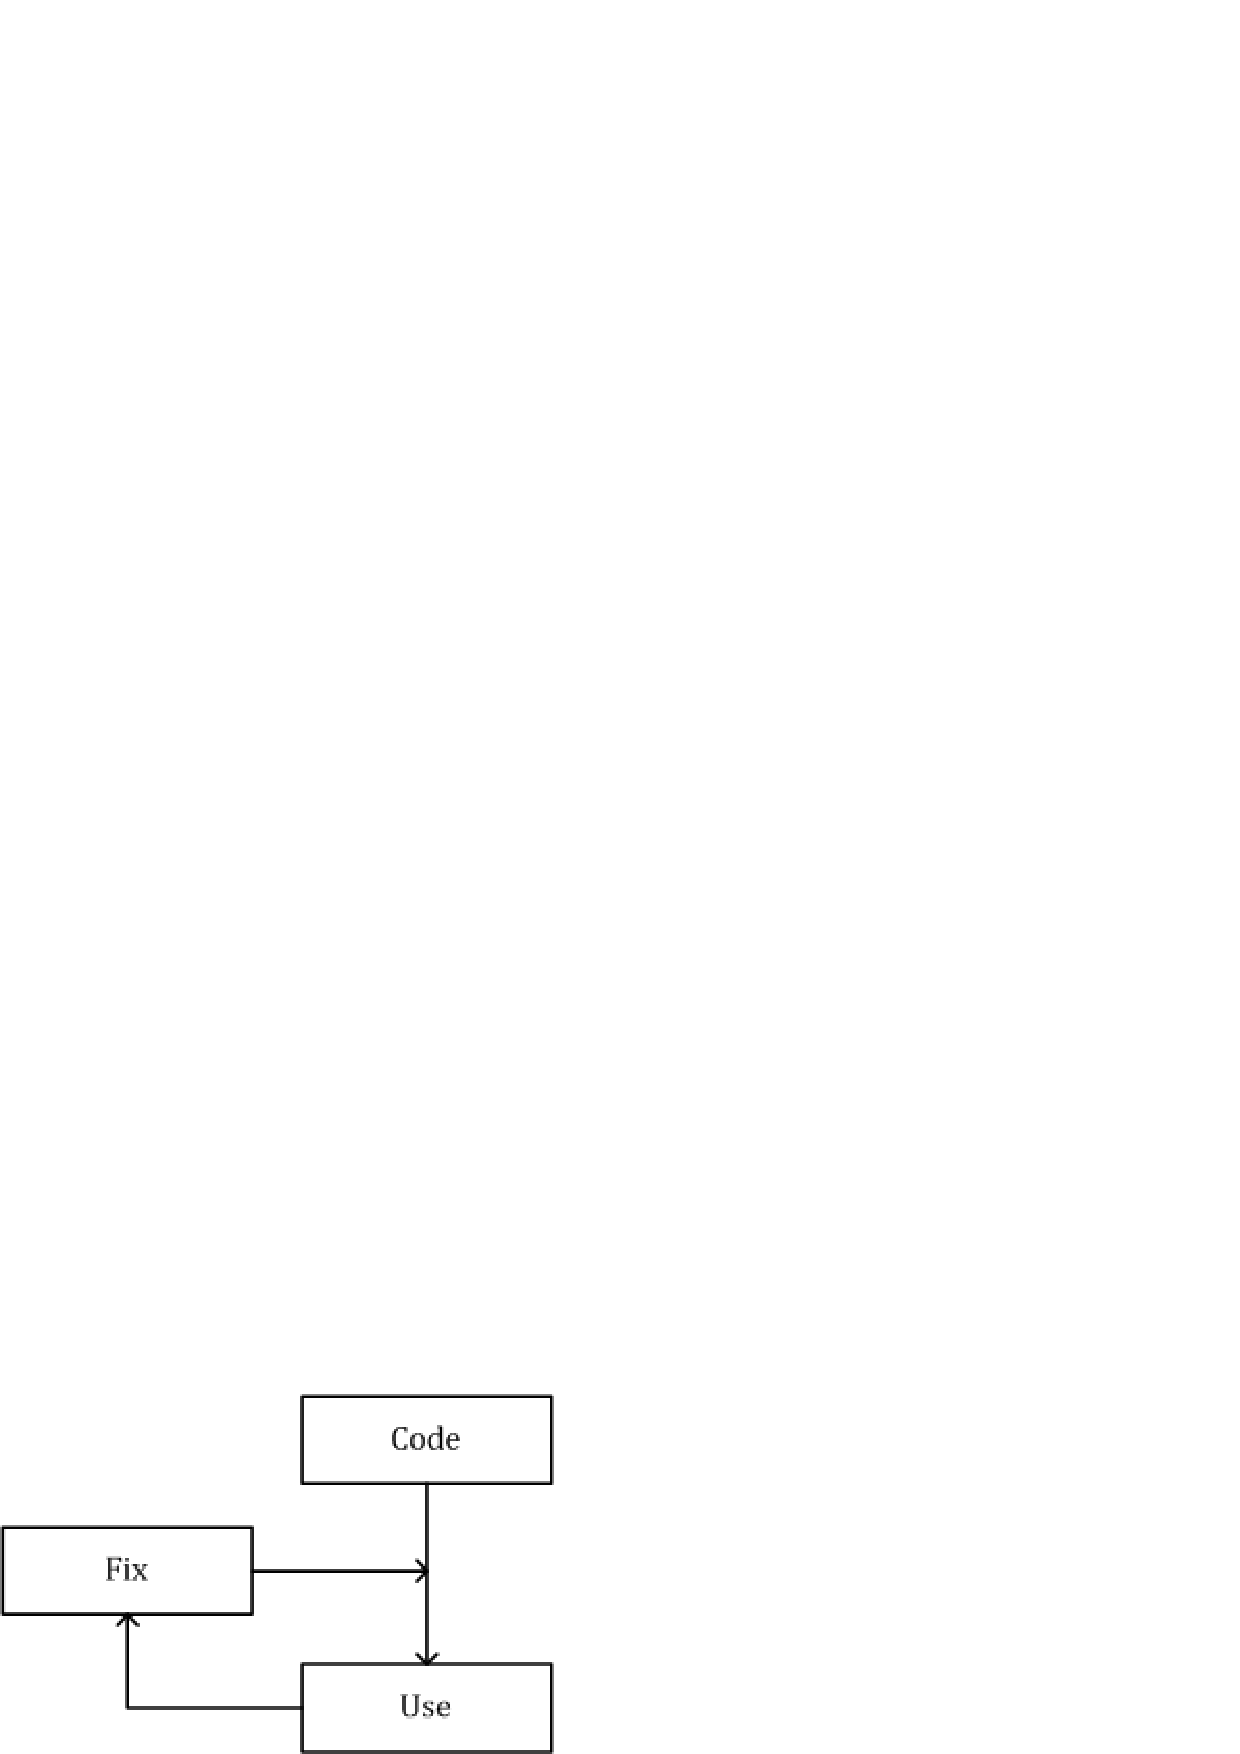
\includegraphics[height=60mm]{model_00_code_and_fix}
   \caption{The code-and-fix model \cite{citeulike:10002126}.}
   \label{fig:code_fix_model}
\end{figure}

\section{Stagewise model}
Through the experience with code-and-fix approach the need for requirements collection and 
for the distinct design phase prior to coding become evident, as well as the need of structured 
testing and evaluation. The recognition these needs by the industry, and the first experiences
with development of large software systems such as Semi Automated Ground 
Environment \cite{citeulike:10004001} \cite{citeulike:10004037} led to the development 
of stagewise software model by Benington (1956) \cite{citeulike:10004032}. 
This model consisted of a number of stages:
\begin{itemize}
 \item Operational plan
 \item Operational specifications
 \item Coding specifications
 \item Coding
 \item Parameter testing
 \item Assembly testing
 \item Shakedown
 \item System evaluation
\end{itemize}
These stages were streamlined as a sequential process - every completed stage created a
grounds for its successor. While now seems to be naive and straightforward, this very 
first formalization of the software process was a significant breakthrough at the time. 
But soon it was recognized, that this unidirectional process does not stipulate what 
has to be done if the rework of previous stage(s) is necessary - there was 
no formalization of such backward transitions and the revision of the model was requested.

\section{Waterfall model}
The waterfall model was a refinement of a stagewise model and its original version is 
credited to Royce (1970) \cite{citeulike:9982731}. This is probably the oldest of living
models as well as the most influential one. It is still very popular in the domain of 
development of large and complex software systems. 

The waterfall model has two major changes from the predecessor - first is the recognition 
of the feedback loops between stages and second is the inclusion of a prototyping stage. 
There is a limitation imposed on the backward transitions for successive stages only - 
in order to exclude expensive cross-stage rework \cite{Boehm95anchoringthe}.

\begin{figure}[tbp]
   \centering
   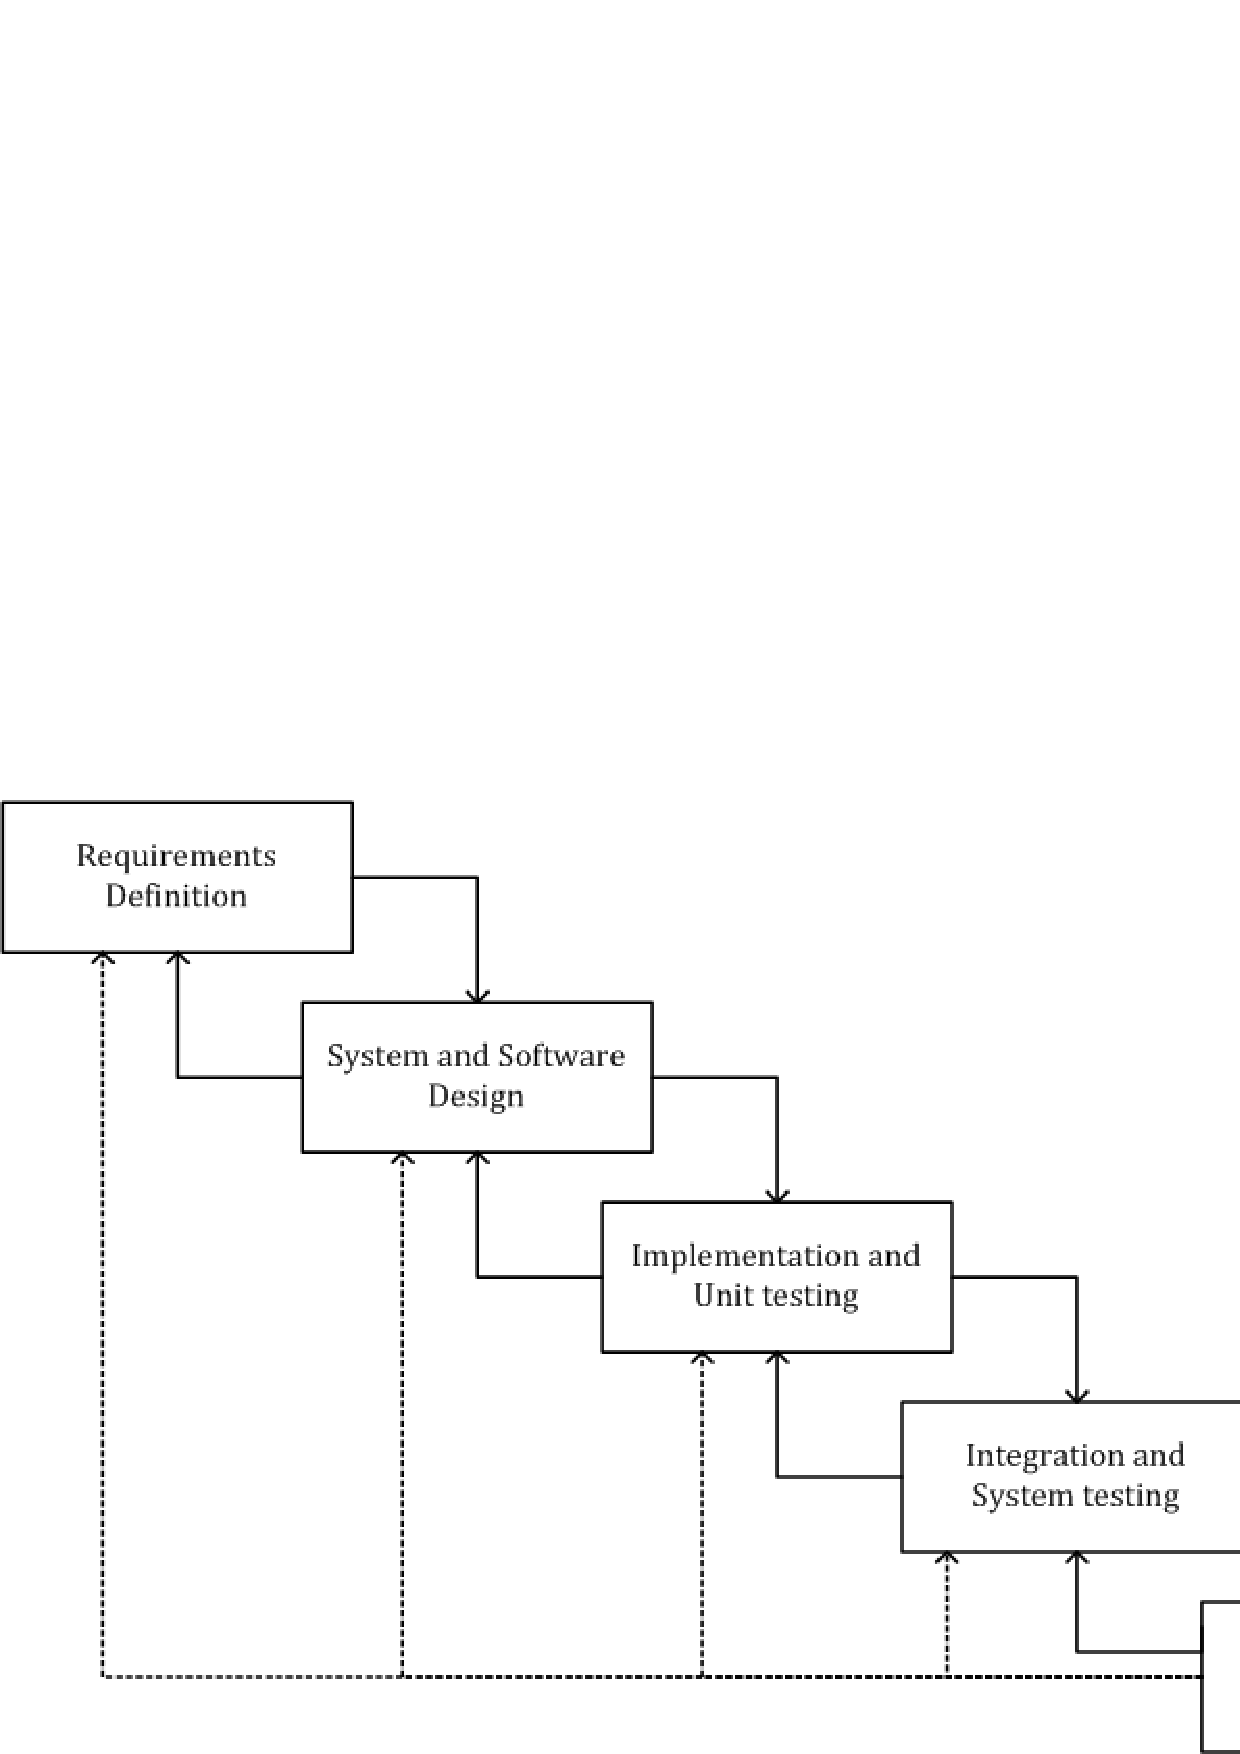
\includegraphics[height=87mm]{model_01_waterfall}
   \caption{The waterfall software development model. Solid lines represent a staged 
      model implementation with no feedback. Dotted lines add a possibilty of 
      iterative transition between adjacent stages. Dashed line show model 
      implementation with feedback \cite{citeulike:9982731}. }
   \label{fig:model_waterfall}
\end{figure}

Five stages of waterfall model depicted on the figure \ref{fig:model_waterfall} 
reflect the fundamental development activities:
\begin{enumerate}
 \item \textit{Requirements analysis and definition.} 
The feasibility study is conducted and the requirements collected. 
The system functionality clarified and documented in details - the requirements 
specification document delivered  and will serve as the system specification. 
It is assumed that the customer's expectations are articulated and will not 
change much throughout the development process.
 \item \textit{The system design.} 
Within this phase requirements for hardware and software components are defined 
by establishing the overall system architecture. All system modules and their 
interactions are designed in accordance with collected requirements.
 \item \textit{Implementation and unit testing.} 
The actual code produced, system modules are tested individually. 
This phase embeds all quality control checks.
 \item \textit{Integration and system testing.} 
System components assembled together. Complete system is tested and evaluated in 
actual production conditions (alpha tested).
 \item \textit{Delivery and Maintenance.} 
System is tested by actual customer (beta testing). Identified errors are corrected 
and if found satisfiable, software system is installed and put into use. 
Maintenance involving error correction and system improvements along with functionality 
enhancements is carried on.
\end{enumerate}

As we can see, there is successive and distinct progression of stages in waterfall model;
each of the states is well defined and forms a basis for a successive one. 
Each state has milestones and deliverables explicitly defined in the specification documents.
In addition to this deliverables, each of the stages producing a document 
which describes what exactly occurred within this stage providing a process visibility 
and facilitating audit. 

The big advantage of waterfall model of software development process is that 
it is consistent with other engineering models in terms of general approach, 
its flow and produced documentation. 
It is manager-friendly as well since it is possible to track the project progress 
against the written development plan. 
The major problem hovewer is that within this upfront specification based approach 
stakeholders finding it extremely difficult to articulate their requirements in advance and 
that requirements changes are very hard to incorporate after first stages are passed.

During transition from stage to stage within the waterfall model, previous state 
should be signed-off - approved to be in finished state. In other 
word, states should not overlap, however in the real life problems often discovered
later on - for example it is often happens that problems with design 
discovered only after implementation is started and so on. In such situation
process returns to the problematic phase and changes are made and reflected in 
the documentation. These iterations are very costly in time and effort and 
usually after a certain number of iterations problematic stages considered 
``frozen'' and development continues. Identified and not resolved issues persist
through the further work and if possible - covered by workarounds, if not - 
they just ignored and system may not perform correctly or lack some functionality 
afterwards.

Waterfall model is an example of a plan-driven process - one must plan and schedule all 
of the activities upfront their execution. The waterfall model has many variations and 
the general waterfall-like approach forms the basis of many standards in the software industry.

In 1988 Boehm revisits waterfall model and after re-stating its fundamental problems 
offers three classes of improved software process models - evolutionary development 
model, the transform model and the spiral model \cite{citeulike:10002126}.

\subsection{Evolutionary development model}
Evolutionary development proposed by McCracken\&Jackson in 1982 \cite{citeulike:3996892}
was among the first reactions to the waterfall model's problems. Instead of moving 
through well-defined stages and producing number of documents, it claims the only
stage - release of extended system capability which is a response to the user 
requirements and is based on the operational experience. Evolutionary paradigm 
is built around early release of the pre-operational product (prototype) and its gradual 
enhancement (evolutional development) through feedback. 

Within the evolutionary development model stakeholders are provided with a somewhat 
functioning software system at the very beginning and their feedback directs all future
software system enhancements. This model perfectly matches the user expectations 
about the software requirements evolution - gradually, through everyday experiences, 
as an opposite to waterfall model upfront requirements collection. 

However, this is what fails in evolutionary development - the new model was found 
stigmatized with weaknesses of the old code-and-fix approach - spaghetti code and 
the lack of formal planning - the exact reasons waterfall model was invented... 
And in addition evolutionary development does not provide any means for identifying 
and fixing early erroneous design decision - instead it encourages working around 
major issues which inevitably creates large expensive to maintain codebase instead 
of re-considering early decisions.


\subsection{Spiral model}
The spiral model reflects the concept in which each of development cycles involves a 
progression addressing the same sequence of steps as in previous level. The figure 
\ref{fig:model_spiral} illustrates the model representation as a spiral according 
to Boehm \cite{citeulike:10002126}. Each loop of this spiral represents a phase of 
software process. Innermost loop concerns the system feasibility study. The second 
loop represents a system requirements definition and system design and so on. 
The radial (Y) dimension represents a cumulative cost of the system up to date, 
while angular dimension represents a loop progress towards completing the current 
spiral loop.

\begin{figure}[tbp]
   \centering
   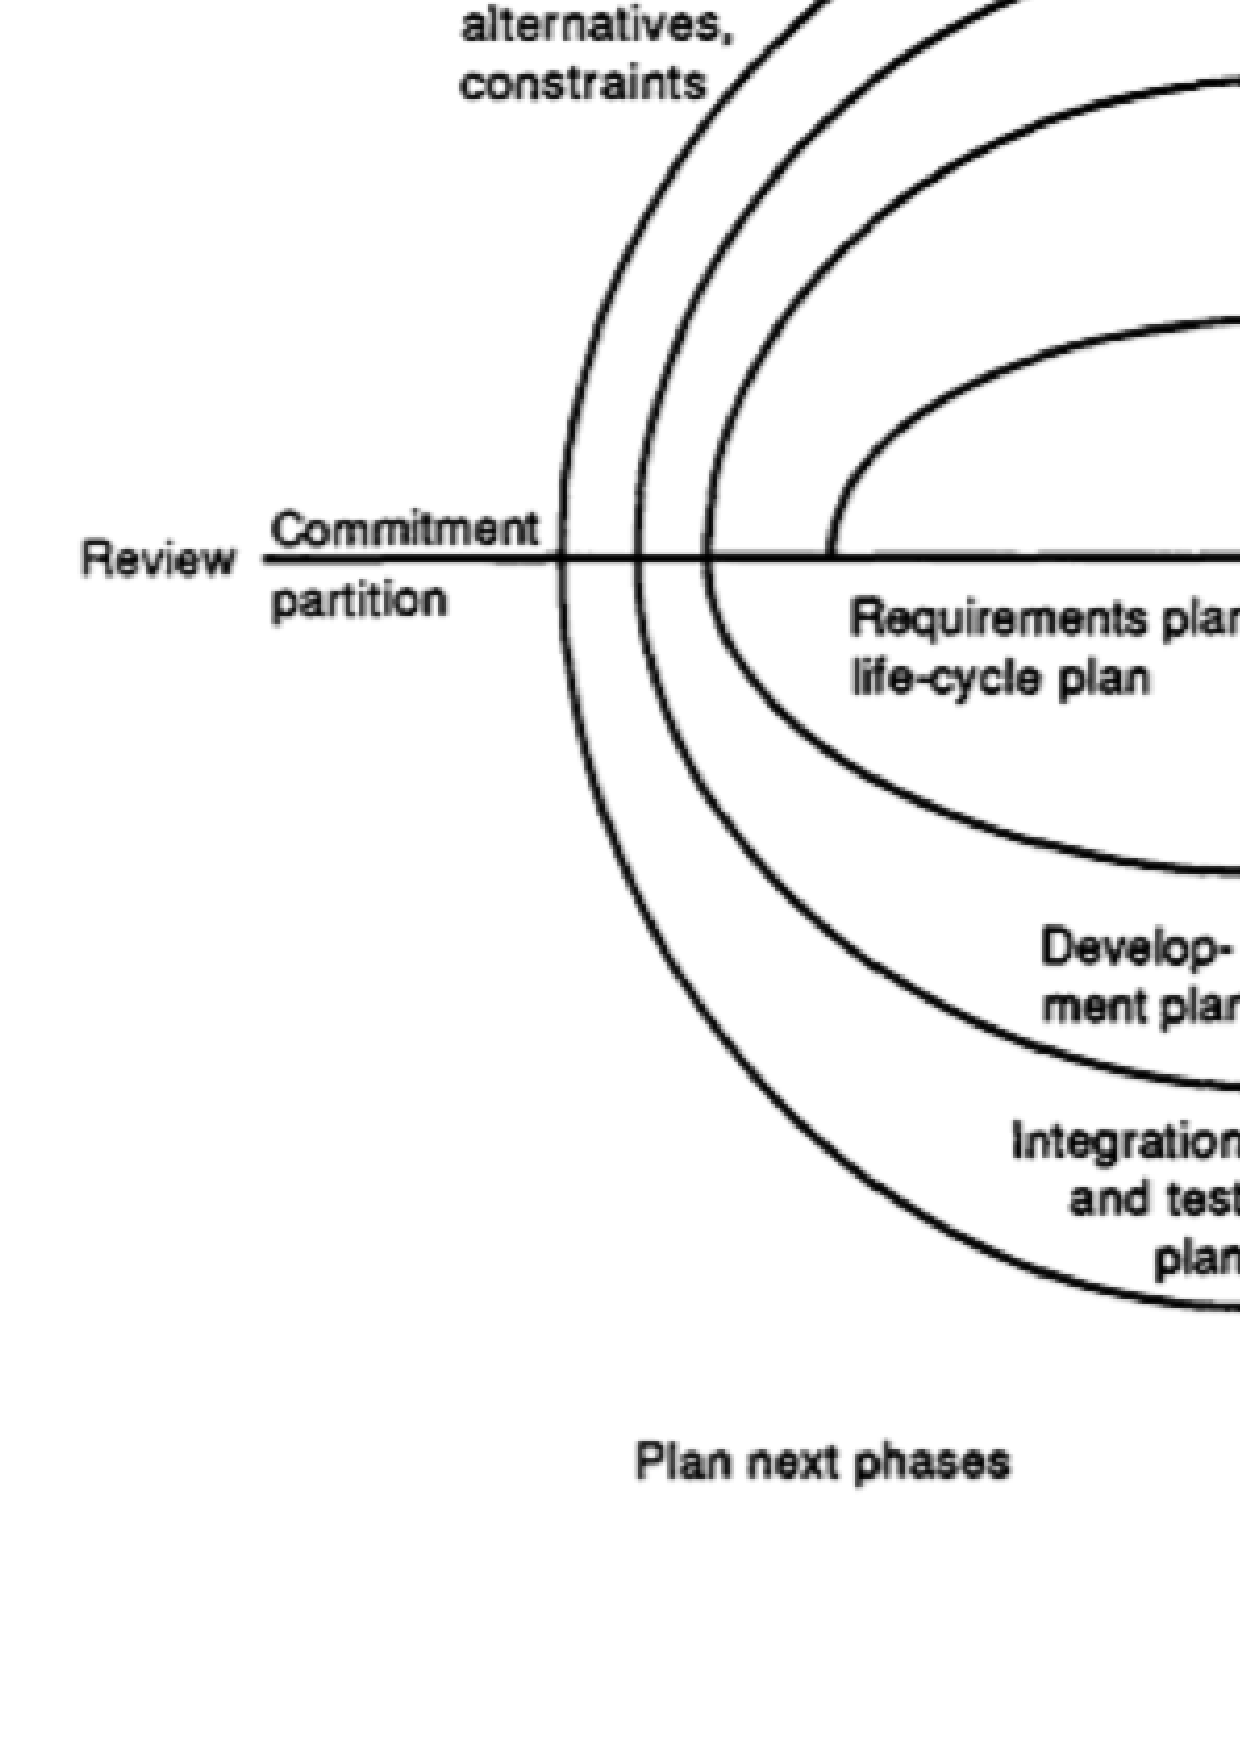
\includegraphics[height=150mm]{model_02_spiral-boehm}
   \caption{The spiral model of software development according to Boehm \cite{citeulike:10002126}. }
   \label{fig:model_spiral}
\end{figure}



\subsection{Cleanroom software engineering}
Another of waterfall model derivatives is a Cleanroom development methodology, which is
a fusion of waterfall model with formal methods approach. 
Following the formal methodology, stages of waterfall model reshaped into 
\begin{enumerate}
 \item \textit{Formal specification} phase, where the software system is presented as 
a state-transition model with input and output. The states of the system and
its transitions (reactions on input) reflect specification and requirements.
 \item \textit{Structured, incremental development} phase. By application of the 
cleanroom methodology the software is partitioned into increments using the 
specification and the development process Within cleanroom
development process only a limited amount of programming constructs allowed,
and the development process is an iterative refinement of specification
\end{enumerate}

1) formal specification phase; 2) incremental, formal development and verification 
, formal methods are a particular kind of mathematically-based techniques for
the specification, development and verification of software and hardware systems

\section{}

It is currently well recognized in the software industry that the process of software development 
is critical to the success of any major development project.
The Institute of Electrical and Electronics Engineers defines software engineering as 
“the application of a systematic, disciplined, quantifiable approach to development, 
operation, and maintenance of software; that is, the application of engineering software”
